\section{Architectural Design}

%  in automatico Section [number]
\subsection{Overview}
\begin{figure}[H]
          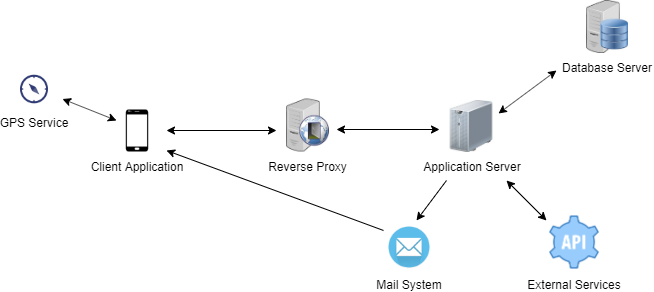
\includegraphics[scale=0.54,left]{Images/overview.png}
        \caption{System overview}
\end{figure}
The above figure shows an high level overview of the System's architecture.\\
We can immediately identify that is divided in two parts: the Client Application part and the Application Servers part.\\
The former shows the services used by the Client Application and its communication with the Application Servers.\\
The other one indicates how the System work with the external functionalities in order to accomplish the required Goals.\\
Further details on the System components and their interactions will be explained in detail in the following sections.

\subsection{Component view}

\subsection{Deployment view}
The distribution of components capturing the topology of the system is illustrated below by using a deployment diagram.\newline
The system is structured in a multitier architecture.
\newline
\begin{figure}[H]
          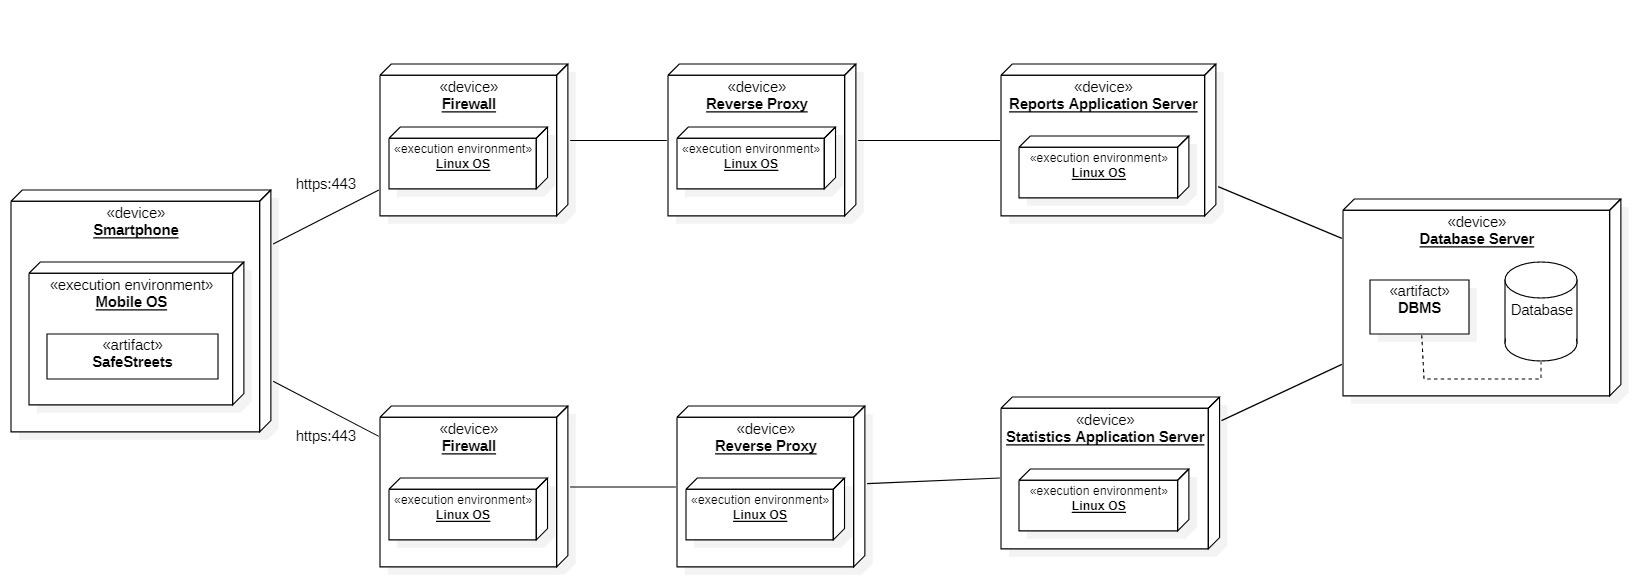
\includegraphics[width=1.25\textwidth,left]{Images/deployment_diagram.png}
        \caption{Deployment Diagram}
\end{figure}
\noindent\textbf{Smartphone}\newline
This node represents the smartphone of the User or Authority, both can access to the functionalities of SafeStreets by using their own smartphone.
\newline
\textbf{Firewall}\newline
This component allows to protect the Reverse Proxy by filtering the packets received from \textit{internet}.
\newline
\textbf{Reverse Proxy}\newline
We chose to deploy a reverse proxy in order to increase parallelism and scalability. Moreover, the reverse proxy is responsable of the load balancing since the component receiving all the request from internet (filtered by the Firewall). Another reason for the deployment of The Reverse Proxies is because it increases security and anonymity by protecting the identity of our backend servers.
\newline
\textbf{Receiver Application Server}\newline
This component contains all the logic used to receive reports from Users and the forwarding of those to the corresponding Authorities. This component may also be replicated in order to balance the workload.
\newline
\textbf{Statistics Application Server}\newline
In order to decouple all the logic behind the functionalities offered by SafeStreets, it has been decided to use a seperate Server that allows to compute satistics by accessing to local information and municipalities' public information.
\newline
\textbf{Database Server}\newline
This part of the System is equipped with a relational DBMS, it allows to store and retreive all the data needed by the Application Servers.

\subsection{Runtime view}

\subsection{Component interfaces}

\subsection{Selected architectural styles and patterns}

\subsection{Other design decisions}